\documentclass{beamer}
\usepackage{beamerthemesplit}
\usepackage{wrapfig}
\usetheme{SPbGU}
\usepackage{pdfpages}
\usepackage{amsmath}
\usepackage{mathtools}
\usepackage{cmap} 
\usepackage[T2A]{fontenc} 
\usepackage[utf8]{inputenc}
\usepackage[english,russian]{babel}
\usepackage{indentfirst}
\usepackage{amsmath}
\usepackage{tikz}
\usepackage{multirow}
\usepackage[noend]{algpseudocode}
\usepackage{algorithm}
\usepackage{algorithmicx}
\usepackage{ stmaryrd }
\usepackage{qtree}
\usetikzlibrary{shapes,arrows}
\usepackage{fancyvrb}
\usepackage{minted}
\newtheorem{rutheorem}{Теорема}
\newtheorem{ruproof}{Доказательство}
\newtheorem{rudefinition}{Определение}
\newtheorem{rulemma}{Лемма}
\beamertemplatenavigationsymbolsempty

\newcommand{\derive}[0]{\xRightarrow[]{*}}
\newcommand{\derives}[0]{\xRightarrow[]{}}
\newcommand{\derivek}[1]{\xRightarrow[]{#1}}
\newcommand{\deriveg}[1]{\xRightarrow[#1]{*}}
\newcommand{\derivegone}[1]{\xRightarrow[#1]{}}

\title[]{Теория автоматов и формальных языков}
\subtitle[]{Магазинные автоматы}
\institute[]{
Санкт-Петербургский государственный электротехнический университет <<ЛЭТИ>>\\
}

\author[]{Екатерина Вербицкая}

\date{15 ноября 2016г.}

\definecolor{orange}{RGB}{179,36,31}

\begin{document}
{
  \begin{frame}
    \titlepage
  \end{frame}
}

\begin{frame}[fragile]
  \transwipe[direction=90]
  \frametitle{В предыдущей серии}
  \begin{itemize}
    \item Регулярные языки распознаются с помощью конечных автоматов
    \item Разные алгоритмы синтаксического анализа для контекстно-свободных языков
    \begin{itemize}
    	\item CYK
    	\item Эрли
    	\item Рекурсивный спуск
    	\item LL(1)
    	\begin{itemize}
    		\item GLL
    	\end{itemize}
    	\item LR(0), SLR(1), CLR, LALR(1)
    	\begin{itemize}
    		\item GLR
    	\end{itemize}
    \end{itemize}
    \item Есть ли универсальный распознаватель для КС-языков?
  \end{itemize}
\end{frame}

\begin{frame}[fragile]
  \transwipe[direction=90]
  \frametitle{TLDR}
  \begin{itemize}
  	\item Произвольный КС язык можно распознать при помощи магазинного автомата (он же автомат с магазинной памятью, он же pushdown automata, он же pda)
  	\item Магазинный автомат по сути --- автомат со стеком
  	\item Детерминированные магазинные автоматы могут распознавать только детерминированные КС языки
  	\item Недетерминированные магазинные автоматы могут распознавать произольные КС языки
  \end{itemize}
\end{frame}

\begin{frame}[fragile]
  \transwipe[direction=90]
  \frametitle{Что такое магазинный автомат}
\begin{center}
  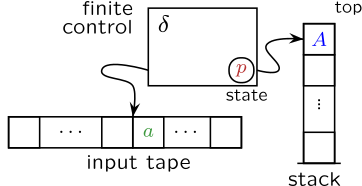
\includegraphics[width=\textwidth]{pics/Pushdown.png}
\end{center} 

\end{frame}

\begin{frame}[fragile]
  \transwipe[direction=90]
  \frametitle{Что такое магазинный автомат: неформально}
\begin{itemize}
	\item Автомат, переходы которого осуществляются по входному символу, текущему состоянию и символу на вершине стека
	\begin{itemize}
		\item У конечного автомата не было стека
	\end{itemize}
	\item Никакие состояния стека, кроме вершины, не доступны
	\item Во время перехода может изменяться стек
	\begin{itemize}
		\item Положить что-то на стек (push)
		\item Снять верхушку со стека (pop)
	\end{itemize}
	\item А может и не изменяться
	\begin{itemize}
		\item Магазинный автомат может вообще игнорировать стек
		\item Или стек может не изменяться, хоть значение оттуда и читается
	\end{itemize}
	\item Итого: по тройке (входной символ, состояние, символ на вершине стека) получается новое состояние, и модифицируется (или нет) стек
\end{itemize}
\end{frame}

\begin{frame}[fragile]
  \transwipe[direction=90]
  \frametitle{Детерминированные магазинные автоматы vs недетерминированные}
\begin{itemize}
	\item В общем случае одной входной строке может соответствовать несколько вычислений
	\begin{itemize}
		\item Некоторые из них могут завершаться в принимающих состояниях
	\end{itemize}
	\item Если существует хотя бы одно вычисление, завершающееся в принимающем состоянии, строка принадлежит языку
	\item Если для каждой строки существует ровно одно вычисление в магазинном автомате, то он является детерминированным
	\begin{itemize}
		\item Соответсвующий язык является детерминированным КС языком
	\end{itemize}
	\item Детерминированный магазинный автомат является частным случаем недетерминированного, поэтому детерминированные КС языки --- строгое подмножество контекстно-свободных 
\end{itemize}
\end{frame}

\begin{frame}[fragile]
  \transwipe[direction=90]
  \frametitle{Формальное определение}
  Магазинный автомат это набор $(Q, \Sigma, \Gamma, \delta, q_0, Z, F)$
  \begin{itemize}
    \item $Q$ --- конечное множество состояний
    \item $\Sigma$ --- конечное множество символов, входной алфавит
    \item $\Gamma$ --- конечное множество символов, стековый алфавит
    \item $\delta \subseteq Q \times (Z \cup \varepsilon) \times \Gamma \times Q \times \Gamma^*$ --- конечное  подмножество, задающее отношение переходов
    \item $q_0 \in Q$ --- стартовое состояние
    \item $Z \in \Gamma$ --- начальный элемент стека
    \item $F \subseteq Q$ --- множество принимающих (конечных) состояний
  \end{itemize}
\end{frame}


\begin{frame}[fragile]
  \transwipe[direction=90]
  \frametitle{Отношение переходов}
  $(p, a, A, q, \alpha) \in \delta$  означает
  \begin{itemize}
    \item Если магазинный автомат находится в состоянии $p \in Q$, на вершине стека находится $A \in \Gamma$, а со входа читается символ $a \in \Sigma \cup \varepsilon$, то изменяем состояние на $q \in Q$, снимаем со стека символ $A$, записываем на стек строку $\alpha \in \Gamma^*$
    \item $\Sigma \cup \varepsilon$ сигнализирует о том, что вход можно и не читать
    \item Иногда $\delta$ альтернативно определяют как отображение $\delta :: (Q \times (\Sigma \cup \varepsilon) \times \Gamma \rightarrow 2^(Q \times ))$
  \end{itemize}
\end{frame}

\begin{frame}[fragile]
  \transwipe[direction=90]
  \frametitle{Семантика магазинного автомата}
\begin{itemize}
  \item Мгновенное описание МА: $(p, \omega, \beta) \in Q \times \Sigma^* \times \Gamma^*$
  \begin{itemize}
  	\item $p$ --- текущее состояние автомата
  	\item $\omega$ --- непрочитанный фрагмент входного потока
  	\item $\beta$ --- содержимое стека (верхушка записана первой)
  \end{itemize}    
  \item Отношение $\vdash$ на мгновенных описаниях (шаг)
  \begin{itemize}
  	\item Для каждого $(p, a, A, q, \alpha) \in \delta$, верно $(p, a x, A \gamma) \vdash (q, x, \alpha \gamma)$ для произвольных $x \in \Sigma^*, \gamma \in \Gamma^*$
  \end{itemize}
  \item В недетерминированных магазинных автоматах может существовать несколько шагов
  \begin{itemize}
    \item Можно выбрать любой
    \item Если какой-нибудь выбор приведет к успеху, значит, строка распознается
  \end{itemize}
  \item Шаг не определен, если стек пуст
\end{itemize}

\end{frame}


\begin{frame}[fragile]
  \transwipe[direction=90]
  \frametitle{Семантика магазинного автомата: вычисление}
  \begin{itemize}
    \item Вычисление --- последовательность шагов
    \item Начальное мгновенное описание $(q_0, \omega, Z)$
    \item Два варианта окончания работы
    \begin{itemize}
      \item По достижении конечного состояния
      \begin{itemize}
        \item $L(M) = \{ \omega \in \Sigma^* \, | \, (q_0, \omega, Z) \vdash^* (f, \varepsilon, \gamma), f \in F, \gamma \in \Gamma^* \}$
      \end{itemize}
      \item По опустошении стека
      \begin{itemize}
      	\item $N(M) = \{ \omega \in \Sigma^* \, | \, (q_0, \omega, Z) \vdash^* (q, \varepsilon, \varepsilon), q \in Q\}$
      \end{itemize}
      \item Эти варианты эквивалентны: по автомату, завершающемуся по первой схеме, можно посмотроить автомат, завершающийся по второй схеме, и наоборот
    \end{itemize}
    \item $\vdash^*$ --- транизитивно рефлексивное замыкание отношения $\vdash$
  \end{itemize}
\end{frame}

\begin{frame}[fragile]
  \transwipe[direction=90]
  \frametitle{Пример: язык $\{ 0^n 1^n \, | \, n \geq 0 \}$}
\begin{center}
  \includegraphics[width=0.7\textwidth]{pics/Pda-example.png}
\end{center}

Вычисление на строке $0011$:
\begin{itemize}
  \item $(p, 0011, Z) \vdash (q, 0011, Z) \vdash (r, 0011, Z)$ --- провал
  \item $(p, 0011, Z) \vdash (p, 011, AZ) \vdash (q, 011, AZ)$ --- провал
  \item $(p, 0011, Z) \vdash (p, 011, AZ) \vdash (p, 11 AAZ) \vdash (q, 11, AAZ) \vdash (q, 1, AZ) \vdash (q, \varepsilon, Z) \vdash (r, \varepsilon, Z)$ --- успех (по принимающему состоянию)
\end{itemize}

\end{frame}

\begin{frame}[fragile]
  \transwipe[direction=90]
  \frametitle{Пример: язык $\{ 0^n 1^n \, | \, n \geq 0 \}$}
\begin{center}
  \includegraphics[width=0.7\textwidth]{pics/Pda-example.png}
\end{center}

Вычисление на строке $00111$:
\begin{itemize}
  \item $(p, 00111, Z) \vdash (q, 00111, Z) \vdash (r, 00111, Z)$ --- провал
  \item $(p, 00111, Z) \vdash (p, 0111, AZ) \vdash (q, 0111, AZ)$ --- провал
  \item $(p, 00111, Z) \vdash (p, 0111, AZ) \vdash (p, 111, AAZ) \vdash (q, 111, AAZ) \vdash (q, 11, AZ) \vdash (q, 1, Z) \vdash (r, 1, Z)$ --- провал
\end{itemize}

\end{frame}


\begin{frame}[fragile]
  \transwipe[direction=90]
  \frametitle{Построение магазинного автомата по КС-грамматике}
  \begin{itemize}
    \item Интуиция:
    \begin{itemize}
      \item Для каждого нетерминала, заменяем его на стеке на правую часть правила
      \item Для каждого терминала, считываем со входа этот терминал и кладем его на стек
    \end{itemize}
    \item Построение:
    \begin{itemize}
      \item Для каждого правила $A \rightarrow \alpha$ добавляем переход $(1, \varepsilon, A, 1, \alpha)$
      \item Для каждого терминала $a$, добавляем $(1,a,a,1,\varepsilon)$
    \end{itemize}
    \item Относительно бесполезный автомат: как найти правильное вычисление?
  \end{itemize}
\end{frame}

\begin{frame}[fragile]
  \transwipe[direction=90]
  \frametitle{Лемма о накачке для КС языков}
  \begin{rutheorem}
    Если язык $L$ является контекстно свободным, то 
    
    $\exists p \geq 1: \forall s \in L. |s| \geq p $ можно разбить на подстроки $s = uvwxy: |vwx| \leq p, |vx| \geq 1$ и
    
     $\forall n \geq 0. \, u v^n w x^n y \in L$
  \end{rutheorem}
\end{frame}

\begin{frame}[fragile]
  \transwipe[direction=90]
  \frametitle{Лемма о накачке для КС языков: пример}
  Язык $L = \{ a^n b^n c^n \}$
  
  Предполагаем, что он КС, тогда по Лемме существует $p$... 
  
  Рассмотрим слово $a^p b^p c^p = uvwxy, |vwx| \leq p, |vx| \geq 1 $
  
  \begin{itemize}
    \item $vwx = a^j$
    \item $vwx = a^j b^k, j + k \leq p$
    \item $vwx = b^j, j leq p$
    \item $vwx = b^j c^k, j + k \leq p$
    \item $vwx = c^j, j \leq p$
  \end{itemize}   
  
  Строка $u v^i w x^i y $ не содержит одинаковое количество букв для всех $i$. Например, рассмотреть $i = 2$. Получили противоречие --- успех
\end{frame}

\end{document}
